\chapter{Forbidden histories}\label{ch:duality}

The preceding chapters described the \emph{admissible} histories. A rule is, however, naturally specified by what it \emph{forbids}, and the forbidden histories form a complex of their own. By Alexander duality its topology is that of the admissible complex, shifted by one dimension. For rules in which admissibility is decided by prefix sets, a class that contains every arithmetic rule of the Substrate (\cref{lem:F}), the forbidden complex collapses up to homotopy to a small combinatorial complex built from the prefix sets that can never be completed. The question ``is there a two-dimensional hole in $K_A$?'' becomes ``is there a one-dimensional cycle that does not bound in a complex on at most $62$ vertices?''. Homology has coefficients in $\F$, $k=6$ unless stated, and all complexes are finite. Alexander duality, the nerve theorem and Quillen's closure lemma are classical and are used as such.

\section{Flags, prefix sets and two dual spheres}\label{sec:flags}
Let $[k]=\{0,\dots,k-1\}$ and $\Pm$ the set of proper nonempty subsets of $[k]$. A \emph{flag} is a maximal chain $I_1\subset\dots\subset I_{k-1}$ in $\Pm$. Flags correspond bijectively to orderings $(x_1,\dots,x_k)$ of $[k]$ via $I_t=\{x_1,\dots,x_t\}$; $I_t$ is the $t$-th prefix set. Let $T=\Delta(\Pm)$ be the order complex of $\Pm$: its simplices are chains, it is the barycentric subdivision of the boundary of a $(k{-}1)$-simplex, hence a triangulated sphere $S^{k-2}$, and its facets are the flags.

The permutohedron $P_k$ has vertices indexed by orderings and proper faces $F(\pi)$ indexed by ordered partitions $\pi=(B_1|\dots|B_m)$ with $m\ge2$ blocks (\cref{def:faces}). To $\pi$ attach the chain
\[
c(\pi)=\{B_1,\ B_1\cup B_2,\ \dots,\ B_1\cup\dots\cup B_{m-1}\}\in T .
\]
This is a bijection between proper faces of $P_k$ and simplices of $T$; $F(\pi)\subseteq F(\pi')$ iff $c(\pi)\supseteq c(\pi')$; and a flag $f$ is a vertex of $F(\pi)$ iff $c(\pi)\subseteq f$. So $\partial P_k$ and $T$ are dual cell structures on the same sphere (\cref{fig:duality}).
@@def:forbidden@@
@@prop:dict@@

\begin{figure}[ht]\centering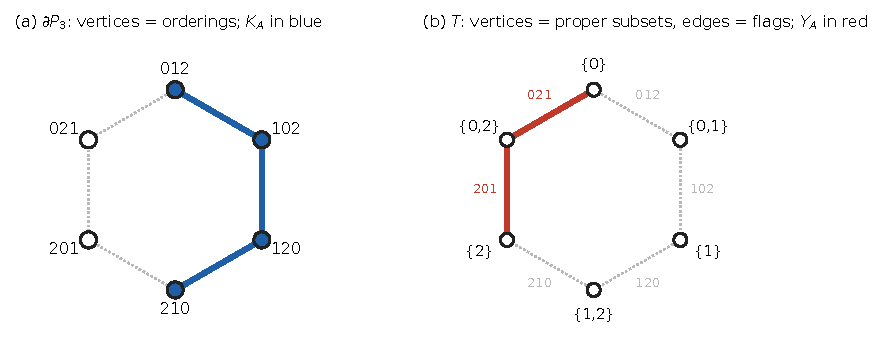
\includegraphics[width=\textwidth]{figures/fig_duality.pdf}
\caption{Duality for $k=3$, where everything can be seen. Left: the hexagon $\partial P_3$ with vertices the six orderings; $A$ consists of four consecutive orderings, and $K_A$ (blue) is the path they span. Right: the dual hexagon $T$, whose vertices are the six proper subsets and whose edges are the flags; $Y_A$ (red) is the subcomplex generated by the two flags of orderings not in $A$. The dictionary of \cref{prop:dict} matches each face of $K_A$ with a simplex of $T$ \emph{outside} $Y_A$. Here $\Hh_0(K_A)=0$ and $\Hh^{0}(Y_A)=0$ because $Y_A$ is connected (the two missing flags share the vertex $\{0,2\}$). Had the two missing orderings been non-adjacent, $K_A$ would have two components and $Y_A$ would be two disjoint edges, so both sides would be one-dimensional.}\label{fig:duality}
\end{figure}

\section{Alexander duality for history complexes}
@@thm:AD+analytic@@
The theorem is why the whole programme can be phrased in terms of forbidden data: \emph{the topology of the history complex is the topology of the forbidden complex}. It explains where $\beta_2$ comes from; the nerve explains how to compute it cheaply.

\section{Dead sets and the nerve theorem}\label{sec:nerve}
@@def:dead@@
Every $I\notin\mathcal A$ is dead, since $I$ is a prefix set of every flag through it, but a set in $\mathcal A$ can be dead too, if every way of completing it passes through a forbidden set. In $N[D]$ two dead sets are joined unless they are complementary, and three form a triangle iff some set is comparable to all of them.
@@lem:quillen@@
@@lem:star+analytic@@
@@thm:nerve+analytic@@
@@cor:dead-cert@@
@@prop:arith-prefix@@

\section{The cycles that carry the holes}\label{sec:cycles}
For a regime the dead sets are computed directly. A triple of dead sets is \emph{hollow} if its three pairs are edges of $N[D]$ (no two complementary) but no set is comparable to all three. A hollow triangle is a $1$-cycle of $N[D]$; it is non-bounding iff it is not a sum of boundaries of triangles.
\begin{figure}[ht]\centering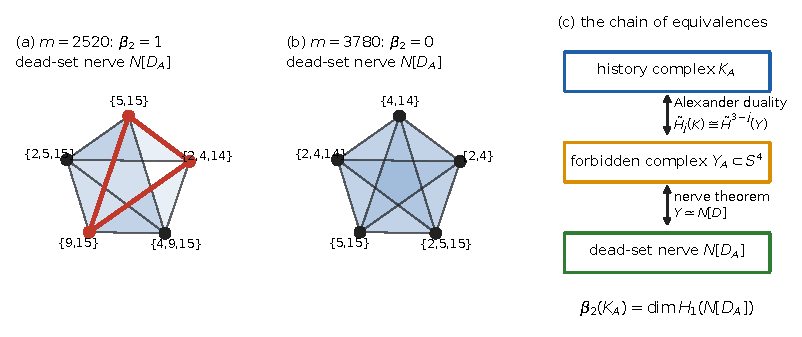
\includegraphics[width=\textwidth]{figures/fig_nerves.pdf}
\caption{Dead-set nerves, recomputed exactly. (a),(b)~Content $(2,4,5,9,14,15)$ at sources $2520$ and $3780$; both systems have $540$ admissible histories and five dead sets and differ in \emph{which} sets are dead. In (a) the red cycle is the hollow triangle $\{2,4,14\},\{5,15\},\{9,15\}$, which does not bound, so $\beta_2=1$; in (b) the nerve is contractible. (c)~The chain of equivalences $\beta_2(K_A)=\dim H_1(Y_A)=\dim H_1(N[D_A])$ (\cref{thm:AD,thm:nerve}).}\label{fig:nerves}
\end{figure}
@@prop:pair+finite-exact@@
The pair at $2520/3780$ is the smallest exhibit: the two systems agree on $N$, $E$, $Q$, $h_1$, $h_q$, $S_B$ and $S_{d2}$ (\cref{ex:pair}) and differ in the radius-two data, but in forbidden-history terms they differ in \emph{which two dead sets} are present, and the nerve cycle is the mechanism.
@@obs:cycle-census+finite-exact@@
In the four census classes with equal $(N,h_1,Q,S_{ds})$ containing both signs, $S_{s2}$ of the positive system is smaller than that of the negative (differences $-16,-16,-16,-48$), and positives have dead sets of smaller size. This is an observation; no derivation of $S_{s2}$ from the nerve is known. Likewise the arithmetic thresholds produce dead sets that are pairwise compatible but have no common comparable set; that is a description of the examples, not an explanation.

\section{Certificates}\label{sec:certificates}
A stand-alone checker (about $200$ lines of Python, standard library only, importing nothing from the research code) recomputes dead sets from the arithmetic definition, builds $N[D]$, checks $\beta_2(K_A)=\dim H_1(N[D])$ from the definition of $K_A$ for four systems, and checks for each of the $290$ stored certificates that $c(\partial\tau)=0$ on every triangle and $c(z)=1$. All checks passed when it was run (\cref{app:status}). The check is sensitive: deleting one cocycle edge from one certificate, or replacing one certificate's cycle by another's, makes it report a failure. The check uses no elimination, only evaluation of the certificate.
